\section{Introduction}
\label{sec:introduction}

The Box Wrapping Problem (BWP) is easy to formulate: given a list of $N \in \Natural$ boxes
$b_i$ each of dimensions $(w_i, l_i)$, where $w_i \in \Natural$ and $l_i \in \Natural$
are the width and length of box $b_i$ respectively, and a roll width $W \in \Natural$,
find the coordinates of  the top-left corner of each box $(\Xtl[i], \Ytl[i])$ so that
the length of roll $L \in \Natural$ is minimised. We call the set of top-left corners, i.e.,
the solution, the placement of all the boxes. In this project we consider only the
2-dimensional case, that is, boxes actually have eight sides that have to be wrapped but,
to make it simple, we consider that a box is just a rectangle. In addition to this, boxes
can be rotated.

\hfill

An example of an instance for this problem is the following: given the list of boxes each
of dimensions $(1,1)$, $(1,1)$, $(2,1)$, $(1,3)$, and $W=3$, find the placement of these
boxes that minimises the roll length. The optimal solution is clearly the one shown
in figure \ref{fig:example-placement}.

\begin{figure}[H]
	\centering
    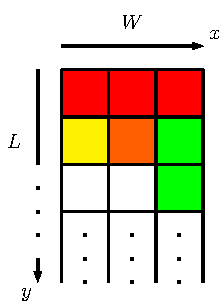
\includegraphics[scale=0.75]{example-placement.pdf}
	\centeredcaption{Optimal placement for $W=3$ and boxes $(1,1)$, $(1,1)$, $(2,1)$,
	$(1,3)$.}
	\label{fig:example-placement}
\end{figure}

There are many ways to solve this problem, but in this project we will solve it from
three different points of view: constraint programming (see section \ref{sec:constraint-programming}),
linear programming (see section\ref{sec:linear-programming}), and satisfiability (see
section \ref{sec:satisfiability}). Since all these approaches require a mathematical modelling
of the problem (variables related by constraints), we give, in section \ref{sec:modelling},
a generic model that should describe the problem well enough to solve it with each technology.
However, each technology may require some extra variables or constraints.